\documentclass{article}
\usepackage{graphicx} 
\usepackage{booktabs} % for formal tables
\usepackage{multirow} % for multirow feature
\usepackage{longtable} % for tables span multiple pages
\usepackage{geometry} % Page margins 
\usepackage{amssymb} %checkmark
\usepackage{pifont} %cross symbol
\usepackage{amsmath} %for math
\usepackage{graphicx} %for figures
\usepackage{hyperref} %cross referencing
\usepackage{textcomp}
\usepackage{natbib}


\title{ME489-HW1}
\author{Batuhan Ülkütaşır}
\date{19 March 2024}

\geometry{left=2cm, right=2cm, top=2cm, bottom=2cm}
\newcommand{\mycheck}{{\ding{51}}}
\newcommand{\mycross}{{\ding{55}}}



\begin{document}
	
	\maketitle
	
	\section{Introduction}
	This paper have been written to demonstrate proficiency in working at LATEX environment as a part of an undergraduate course. All the written content is  based on the article "HORSES3D: A high-order discontinuous Galerkin solver for flow simulations and multi-physics applications." \cite{ferrer2023high} Published at Computer Physics Communications in 24 February 2023.
	\section{Abstract and Overview}
	
	This paper presents a summary of the latest developments of High-Order Spectral Element Solver (HORSES3D), an open source high-order discontinuous Galerkin framework, capable of solving a variety of flow applications, including compressible flows with or without shocks (compressible Navier-Stokes equations), incompressible flows (incompressible Navier–Stokes equations), various RANS and LES turbulence models, particle dynamics, multi-phase flows, aeroacoustics and the Cahn–Hilliard equation and entropy–stable variants are solved. A comparison between high-order solvers widely adopted by industry and academia to simulate fluid flows having comparable capacity with HORSES3D is also included. Regarding the overflow points in the paper, a very detailed documentation and the test cases included in the GitHub repository are discussed. Its innovative approach to solving complex fluid dynamics problems, integrating multiple flow applications into a single framework, sets it apart from other solvers in the field. HORSES3D is a Fortran 2008 object-oriented solver, originally developed to solve the compressible Navier-Stokes equations using DG (high order discontinuous Galerkin) discretisations and explicit time marching.
	
	\subsection{Performance Comparison}
%TABLE İÇİN UNUTMA%
	A range of high-order academic open-source solvers exist and are briefly summarized in Table (\ref{Table1}), where main capabilities are presented. Considering discretisation type, memory versatility and wide range of unique capabilities HORSES3D performs excellently compared to other open-source solvers. It is important to state that commercial products are excluded from the list.
	
		{
			\footnotesize
   \setlength{\tabcolsep}{4.8pt}
			\begin{longtable}{@{}lllllllll@{}}
   
			\caption{Summary of high-order solvers and capabilities.} \label{Table1}\\
			\toprule
			& \textbf{HORSES3D} & {Nek5000} & {Nektar++} & {Semtex} & \text{deal.II} & \text{Flexi/Fluxo} & \text{Trixi.jl} & \text{PyFR} \\ 
			\midrule   
			\textbf{References} & & [11] & [12,13] & [14] & [15] & [16,17] & [18,19] & [20] \\
			\textbf{Language} & Fortran & Fortran & C++ & C++ & C++ & Fortran & Julia & Python \\
			\textbf{Spatial discretisation} & DG & CG & CG/DG & CG & DG & DG & DG & FR \\
			\textbf{Incompressible} & \mycheck & \mycheck & \mycheck & \mycheck & \mycheck & \mycross & \mycross & \mycheck \\
			\textbf{Compressible} & \mycheck & \mycross & \mycheck & \mycross & \mycheck & \mycheck & \mycheck & \mycheck \\
			\textbf{Energy/Entropy stable} & \mycheck & \mycross & \mycross & \mycross & \mycross & \mycheck & \mycheck & \mycross \\
			\textbf{p-adaptation}  & \mycheck & \mycross & \mycheck & \mycross & \mycheck & \mycheck & \mycross & \mycheck \\
			\textbf{Steady/Unsteady}  & S/U & U & S/U & U & S/U & U & U & S/U \\
			\textbf{LES} & \mycheck & \mycheck & \mycross & \mycheck & \mycross & \mycheck & \mycross & \mycheck \\
			\textbf{RANS}  & \mycheck & \mycheck & \mycross & \mycross & \mycross & \mycheck & \mycross & \mycheck \\
			\textbf{Multiphase}  & \mycheck & \mycross & \mycross & \mycross & \mycheck & \mycross & \mycross & \mycheck \\
			\textbf{Shocks}  & \mycheck & \mycross & \mycheck & \mycross & \mycheck & \mycheck & \mycheck & \mycheck \\
			\textbf{Particles}  & \mycheck & \mycross & \mycheck & \mycross & \mycheck & \mycheck & \mycross & \mycheck \\
			\textbf{Aeroacoustics}  & \mycheck & \mycheck & \mycross & \mycross & \mycheck & \mycheck & \mycross & \mycross \\
			\textbf{Immersed Boundaries}  & \mycheck & \mycross & \mycheck & \mycross & \mycheck & \mycheck & \mycheck & \mycross \\
			\textbf{Parallelisation}  & \mycheck & \mycross & \mycheck & \mycross & \mycheck & \mycross & \mycross & \mycross \\
   \textbf{Shared/Distributed-Memory} & S/D & D & D & D & S/D & D & S/D+GPU & S/D+GPU \\

   
				
			\bottomrule
						
		\end{longtable}
			}
		\subsection{Brief Explanation of Numerical Method}	
		The nodal elements in physical domain is tessellated with non-overlapping curvilinear hexahedral elements, \textit{e}, which are geometrically transformed to a reference element, \textit{el.} This transformation is performed using a polynomial transfinite mapping that relates the physical coordinates $\overset{\rightarrow}{x}$ the local reference coordinates $\xi$. The transformation is applied to (\ref{eq1}) resulting in the following:
		
			\begin{equation}
				\label{eq1}
				Ju_{t} + \nabla_{\xi}  \cdot \overset{\leftrightarrow}{\tilde{F}_e} = \nabla_{\xi} \cdot \overset{\leftrightarrow}{\tilde{F}_e} \
			\end{equation}
			where \textit{J} is the Jacobian of the transfinite mapping, $\nabla_{\xi}$ is the differential operator in the reference space and $\overset{\leftrightarrow}{\tilde{F}}$ are the contravariant fluxes for each hexahedral element.	
			After integrating the equation in (\ref{eq1}) to obtain weak form, first by integration parts then coupling with Riemann fluxes $\overset{\leftrightarrow}{\tilde{F}^{*}_{e}}$ a simplified volume form obtained in equation (\ref{eq2}):
		\begin{equation}
			\label{eq2}
			\int_\textit{el} Ju_{t} \cdot \phi_{j} + \int_{\delta\textit{el}} \overset{\leftrightarrow}{\tilde{F}^{*}_{e}}\cdot \overset{\leftrightarrow}{\tilde{F}_e}\phi_{j} - \int_\textit{el} \overset{\leftrightarrow}{\tilde{F}_e} \cdot \nabla_{\xi}\phi_{j} = \int_\textit{el} \nabla_{\xi} \cdot  (\overset{\leftrightarrow}{\tilde{F}_v}) \cdot \phi_{j}  \
		\end{equation}
		As briefly mentioned in the overview part, HORSES3D can operate on aeronautics by using a direct approach and acoustic analogies. In particular, the Ffowcs-Williams and Hawkings (FWH) aeroacoustic analogy is implemented. As a part of this analogy a brief set of equations regarding the acoustic pressure $p=p-p_{0}$ can be obtained from the density fluctuation, as $p=c^{2}_{0}\rho$ in the far field (where $\frac{\rho}{\rho_{0}}<<1$).
		\begin{equation}
  \label{eq3}
			4\pi p_T = \int_S \left[\frac{(1 - M_0 iR_i) \dot{Q}_{i} n_i}{R^*}\right]_{\tau_{e}}\, dS - \int_S \left[ \frac{U_{0i}n_i\hat{R}^*_i Q_{i}}{R^{*2}} \right ]_{\tau_{e}} \, dS,
		\end{equation}
		\begin{equation}
  \label{eq4}
			4\pi p_L = \int_S \left[\frac{\dot{L}_{ij}  n_j\hat{R}_i}{{c_0 R^*}}\right ]_{\tau_{e}} \, dS + \int_S \left[\frac{\dot{L}_{ij} n_j \hat{R}^*_i}{{R^{*2}}}\right ]_{\tau_{e}} \, dS,
		\end{equation}
		In the equations (\ref{eq3}) \& (\ref{eq4}) where $p_T$ is the thickness pressure fluctuation, $p_L$ is the loading pressure fluctuation, $c_0$ is the speed of sound, $M_0$ is the free-stream Mach number, $U_0$ is the free-stream velocity, $R$ is the phase radius, $R^*$ the amplitude radius, and the hat ($\hat{}$) of both $R$ and $R^*$ represents the partial derivatives of the radius quantities. The subscript $\tau_e$ indicates that the integrals are calculated at the emission retarded time.
  

		\subsection{Adaptation}
		The truncation error adaptation algorithm performs mesh p-adaptation for steady and unsteady simulations. Regarding in this topic,	In Fig.(\ref{figure1}) an example of a p-adapted mesh based on truncation errors is shown. There are more examples of truncation error-based adaptation for the compressible Navier-Stokes equations where the contours indicate an average polynomial order.
  
  Moreover, the adaptation process inherently involves a critical decision-making step where the user must select an appropriate target truncation error threshold for the adapted mesh. This selection is pivotal as it directly influences the quality and reliability of the simulation outcomes. Historically, the choice of this threshold has been somewhat contentious, primarily because it lacks a straightforward physical or engineering interpretation, making it a notable drawback of the method.
   
  \begin{figure}[htbp]
			\centering
			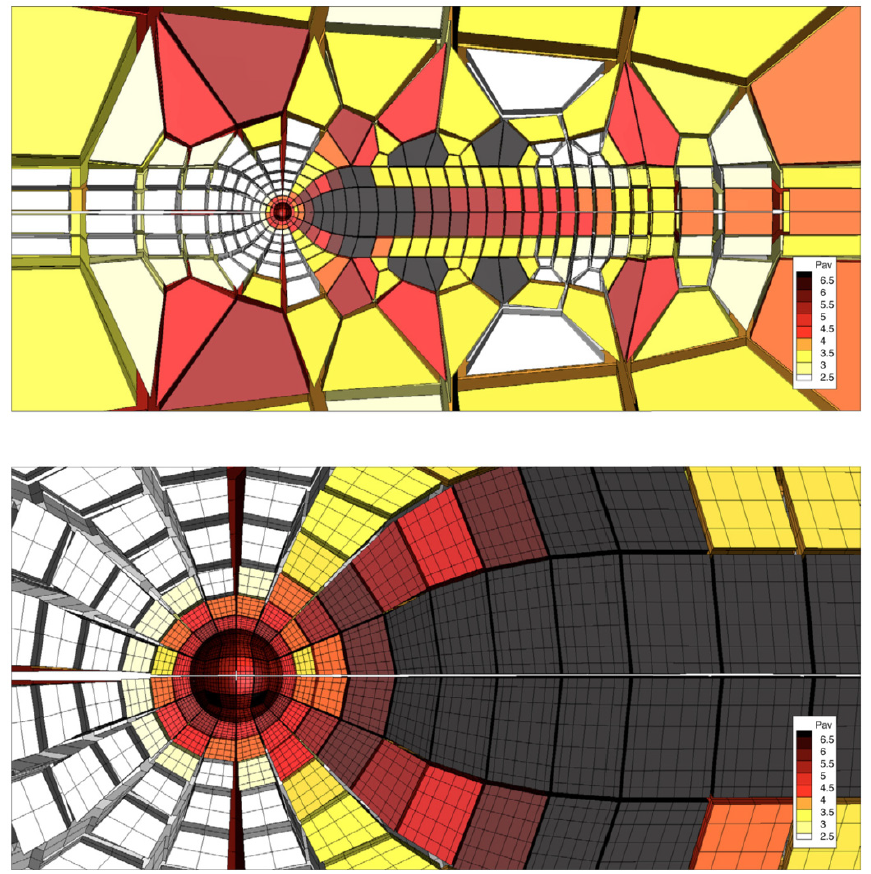
\includegraphics[scale=0.6]{HW1/fig4.PNG}
			\caption{Example of a p-adapted mesh for the flow around a sphere at Reynolds Number 200. The contours indicate the average polynomial order ($P_{av} =(P_x+P_y+P_z)/3$). Figure at the bottom shows zoomed view near the sphere wake region. Retrieved from \cite{ferrer2023high}.}
			\label{figure1}
		\end{figure}
		
		\subsection{Solver Efficiency}
		To reduce the computational cost, all techniques are parallelized for hybrid systems to run on multiprocessor CPUs combining MPI and OpenMP (Shared Memory). To run explicit test on numerical methods the TGV problem (Taylor-Green Vortex) has been widely used to report the subgridscale modeling capabilities of ILES approaches and discretisations. In the Fig.(\ref{figure2}) and Fig.(\ref{figure3}) the TGV case is simulated in a $64^3$ mesh with polynomial or-ders of three to six, giving approximately 16 to 90 million of degrees of freedom. They use Gauss–Lobatto interpolation points and Pirozzoli’s split–form, with Roe (convective) and BR1 (diffusive) fluxes. The number of total cores ranges from one to 700, and the number of OpenMP threads when enabled is 48. Simulations were handled in the MareNostrum-3 supercomputer. 
   
  
\begin{figure}[htbp]
  \centering
  % First figure
  \begin{minipage}{0.45\textwidth}
    \centering
    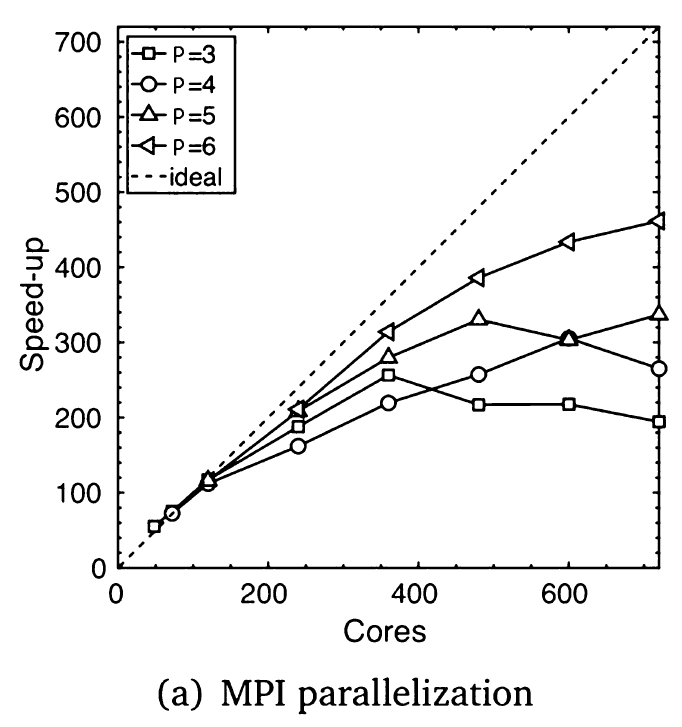
\includegraphics[width=\linewidth]{HW1/figure 5.PNG}
    \caption{HORSES3D scalability solving the TGV problem with a $64^3$mesh using MPIn. Retrieved from \cite{ferrer2023high}.}
    \label{figure2}
  \end{minipage}
  \hfill % Space between the figures
  % Second figure
  \begin{minipage}{0.45\textwidth}
    \centering
    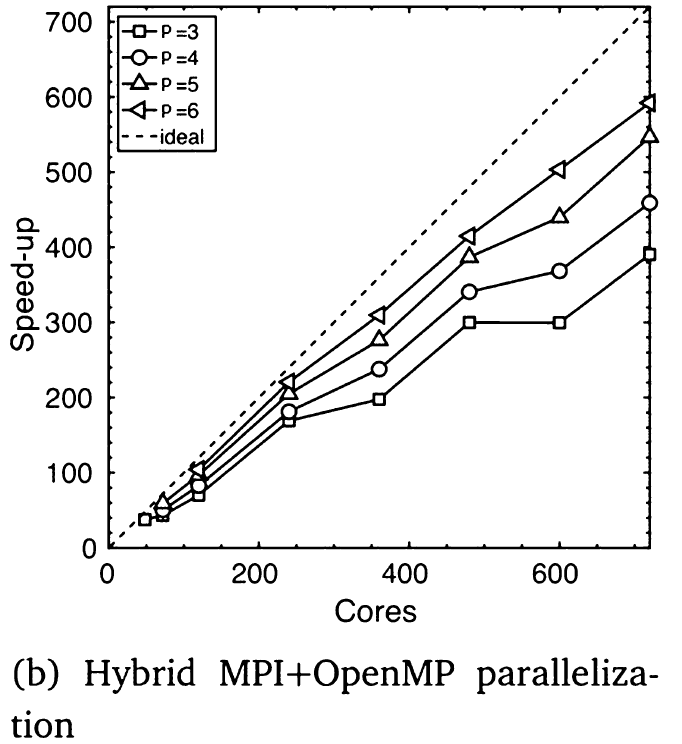
\includegraphics[width=\linewidth]{HW1/figure 6.PNG}
    \caption{HORSES3D scalability solvingthe TGV problem with a $64^3$ mesh using MPI/OpenMP. Retrieved from \cite{ferrer2023high}.}
    \label{figure3}
  \end{minipage}
\end{figure}
  \section{Conclusions and Future Plans}
  HORSES3D is an open-source parallel framework for the solu-tion of non-linear partial differential equations. The solver allows the simulation of compressible flows (with and without shocks), incompressible flows, RANS and LES turbulence models, particle dynamics, multiphase flows, and aeroacoustics. The numeri-cal schemes provide fast computations, especially when selecting high-order polynomials and MPI/OpenMP combinations for a large number of processors. Entropy-stable schemes, local anisotropic p-adaptation, and efficient dual time-stepping and multigrid allow the solver to tackle problems of industrial relevance, such as air-crafts and wind turbines.
  
  HORSES3D is being constantly updated, with the incorporation of neural networks to accelerate simulations and the enabling of connections to external libraries through Python interfaces. Efficiency improvements and expanded simulation capabilities, such as fluid-structure interactions, are being pursued through integration with solvers like MFEM, enhancing both the speed and breadth of applications.
  
\bibliographystyle{plain}
\bibliography{HW1/refhw1}
  
\end{document}
